
\section{Strategy for the $\Hbb$ search}
\label{sec:strategy_Hbb}

This section presents an overview of the analysis strategy adopted in the $\Hbb$ search, which
follows closely that of the previous search performed on the Run 1 dataset~\cite{Aad:2015pja}.

\subsection{Event categorisation}
\label{sec:event_categorisation}

Given the choice of the $W\to\ell\nu$ and $H\to b\bar{b}$ decay modes, the $\ttbar \to WbHq$ signal 
is expected to have four jets in the final state, three of them originating from $b$-quarks, which 
can be effectively exploited to suppress the background. 
Additional jets can also be present because of initial- or final-state radiation.
However, the use of the 60\% $b$-tagging efficiency operating point, characterised by a low mistag rate for
charm and light jets, results in both $\Hc$ and $\Hu$ signals having a similar $b$-tag multiplicity distribution,
with a very small fraction of events having four or more $b$-tagged jets.

In order to optimise the sensitivity of the search, the selected events are categorised into different analysis 
regions depending on the number of jets (4, 5 and $\geq$6) and on the number of $b$-tagged jets (2, 3 and $\geq$4).
Therefore, a total of nine analysis regions are considered:
(4j, 2b), (4j, 3b), (4j, 4b), (5j, 2b), (5j, 3b), (5j, $\geq$4b), ($\geq$6j, 2b), ($\geq$6j, 3b), and ($\geq$6j, $\geq$4b), 
where ($n$j, $m$b) indicates $n$ selected jets and $m$ $b$-tagged jets. 

The overall rate and composition of the $\ttbar$+jets background strongly depends on the jet and $b$-tag 
multiplicities, as illustrated in Figure~\ref{fig:Hbb_Summary}.
Regions with exactly two $b$-tagged jets are dominated by $\ttbar$+light-jets, while regions with 
at least four $b$-tagged jets are dominated by \ttbin. Intermediate compositions are found in regions with exactly three 
$b$-tagged jets.  Most of the $\ttbar$+light-jets background events in these regions have a charm jet from the hadronic $W$ boson 
decay  being $b$-tagged, in addition to the two $b$-jets from the top quark decays.

In the regions with four or five jets and exactly three $b$-tagged jets, which dominate the sensitivity of this search, 
the selected signal events have a $H \to b\bar{b}$ decay in more than 97\% of the events.
The other regions have significantly lower signal-to-background ratios, but they are used for the purpose of improving 
the $\ttbar$+jets background prediction and constraining the related systematic uncertainties
through a likelihood fit to data.  
Because of somewhat larger fraction of $\Hc$ signal in the regions with exactly three $b$-tagged jets,
this analysis is expected to have slightly better sensitivity for $\Hc$ than for $\Hu$ signal.

%%%%%%%%%%%%%%%%%%%%%%%%%%%%%%%%%%%%%%%
\begin{figure*}[t]
\begin{center}
%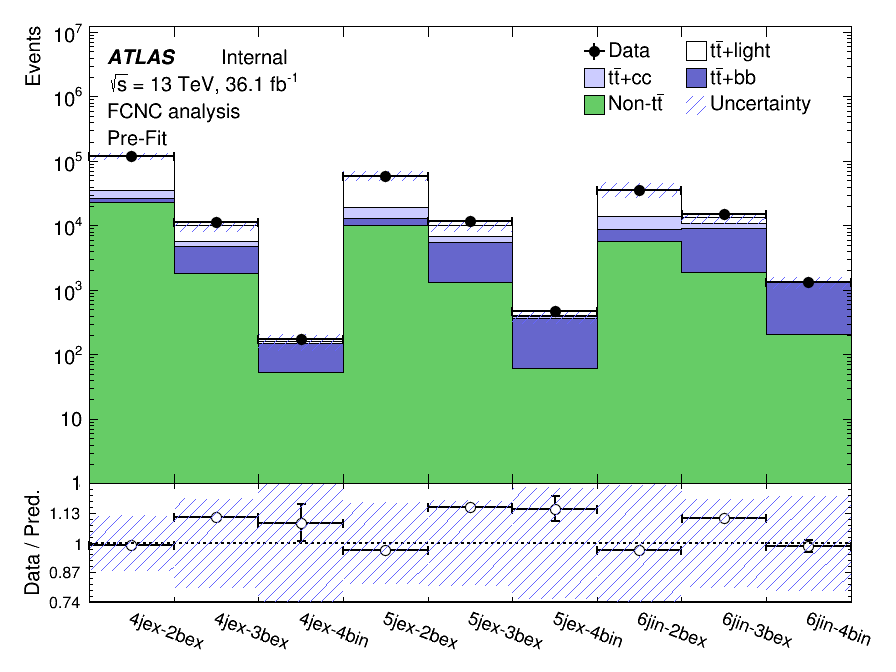
\includegraphics[width=0.55\textwidth]{figures/Hbb/fit/base_ebv2_signal_cH_default_unblinded_splusb/Plots/Summary.png}
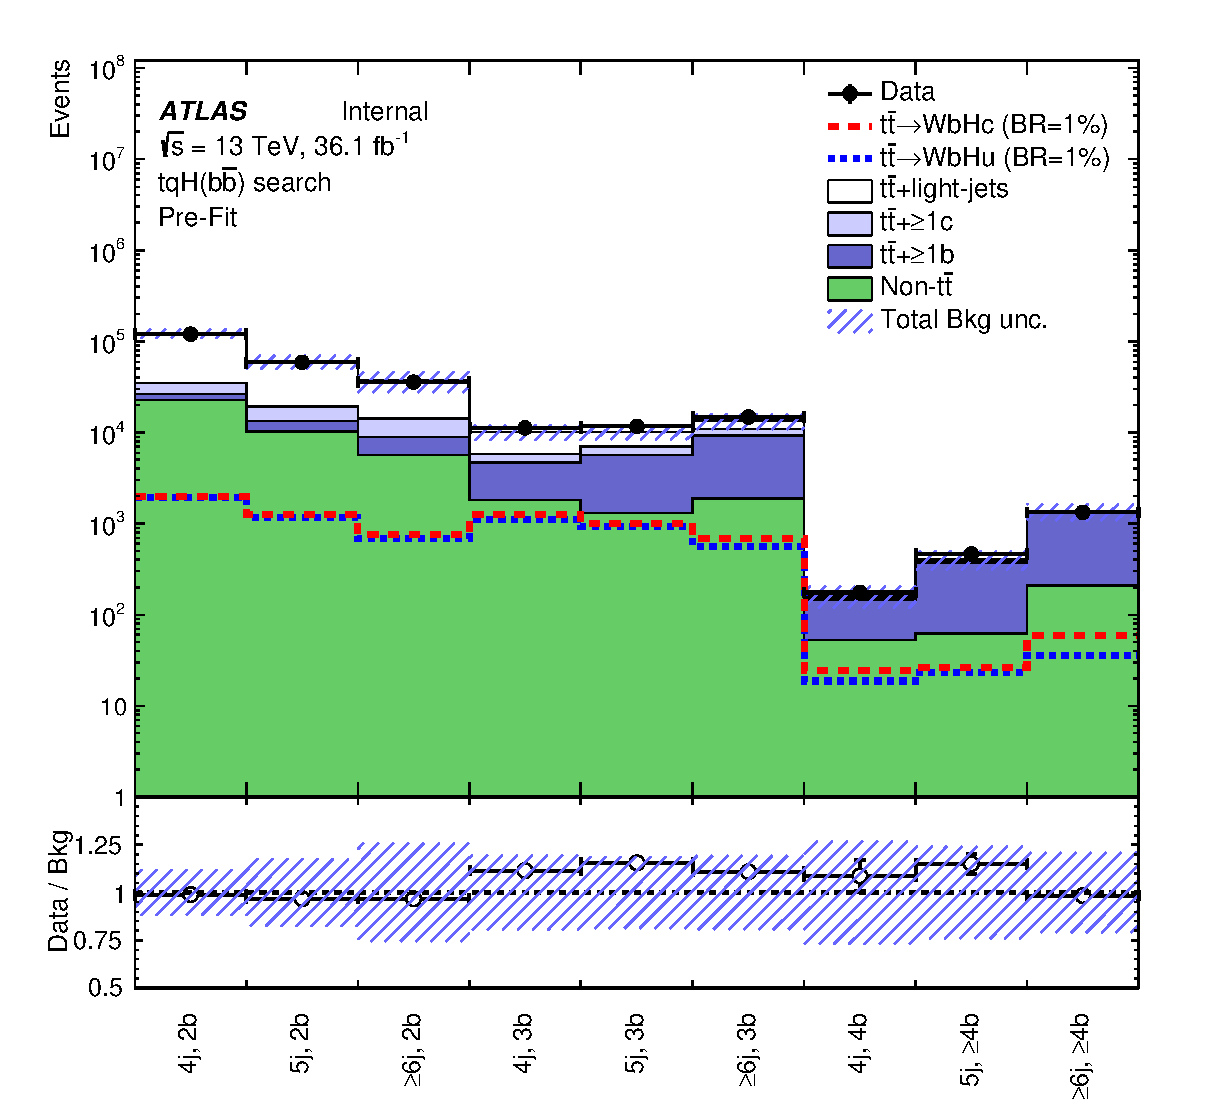
\includegraphics[width=0.55\textwidth]{figures/Hbb/fit/cH_plots/Summary.eps}
\caption{$\Hbb$ search: Comparison between the data and background prediction for the event yields in each of the analysis regions considered 
before the fit to data (``Pre-Fit''). All events satisfy the preselection requirements, whereas those with exactly two $b$-tagged jets are
in addition required to have a value of the likelihood discriminant above 0.6 (see Section~\ref{sec:likelihood_discriminant}).
Backgrounds are normalised to their nominal cross sections.
The small contributions from $W/Z$+jets,  single-top-quark, diboson and multijet backgrounds are combined into a single background source 
referred to as ``Non-$\ttbar$''. 
The expected $\Hc$ and $\Hu$ signals (dashed histograms) are shown separately normalised to $\BR(t\to Hq)=1\%$.
The bottom panel displays the ratio of data to the SM background (``Bkg'') prediction. 
The hashed area represents the total uncertainty of the background, excluding the normalisation uncertainty of the $\ttbin$ background, 
which is determined via a likelihood fit to data.} 
\label{fig:Hbb_Summary}
\end{center}
\end{figure*}
%%%%%%%%%%%%%%%%%%%%%%%%%%%%%%%%%%%%%%%

\subsection{Likelihood discriminant}
\label{sec:likelihood_discriminant}

After event categorisation, the signal-to-background ratio is insufficient even in the best cases to achieve sensitivity, and a suitable
discriminating variable between signal and background needs to be constructed in order to improve the sensitivity of the search.
Since both signal and background result from the $\ttbar$ decay, 
their discrimination is a challenge and it is based on a few measured quantities.  
%there are few experimental handles available to discriminate between them. 
The most prominent features are the different resonances present in the decay (the Higgs boson in the case 
of the $\Hq$ signal and a hadronically decaying $W$ boson in the case of the $\ttbar \to WbWb$ background), and the different flavours of the 
jets forming those resonances. However, the large number of jets in the final state causes ambiguities in the calculation 
of these kinematic variables to discriminate signal events from background events. 

This search uses a similar likelihood (LH) discriminant as that developed in Ref.~\cite{Aad:2015pja}.
The LH variable for a given event is defined as:
\begin{equation*}
LH(\mathbf{x}) = \frac{P^\textrm{sig}(\mathbf{x}) }{P^\textrm{sig}(\mathbf{x}) +P^\textrm{bkg}(\mathbf{x}) },
\label{eq:D}
\end{equation*}
where $P^\textrm{sig}(\mathbf{x}) $ and $P^\textrm{bkg}(\mathbf{x}) $ represent the probability density functions (pdf) of a given event under
the signal hypothesis ($\ttbar \to WbHq$) and under the background hypothesis ($\ttbar \to WbWb$), respectively.
Both $P^\textrm{sig}$ and $P^\textrm{bkg}$ are functions of $\mathbf{x}$, which denotes the set of two-body and three-body invariant masses 
that correspond to the expected resonances in the event (the leptonically decaying $W$ boson, the Higgs boson or the hadronically 
decaying $W$ boson, and the corresponding parent top quarks). These invariant masses are computed from the reconstructed 
lepton, jets, and missing transverse momentum.
As in Ref.~\cite{Aad:2015pja}, $P^\textrm{sig}$ and $P^\textrm{bkg}$ are approximated as a product of one-dimensional pdfs for
each of the invariant masses considered, and averaged among all possible parton--jet matching combinations. 
Combinations are weighted using information on the per-jet multivariate $b$-tagging discriminant value to suppress the impact from 
parton--jet assignments that are inconsistent with the correct parton candidates flavour.

Two background hypotheses are considered, corresponding to the dominant backgrounds in
the analysis: $\ttbar$+light-jets and \ttbin. Thus, $P^\textrm{bkg}$ is computed as the average of
the pdfs for both hypotheses, weighted by their relative fractions found in simulated $\ttbar$+jets events, which depend
on the analysis region considered. Furthermore, in a significant fraction of $\Hq$ simulated events (about 40--50\% in regions with exactly three $b$-tagged jets), 
the light-quark jet from the hadronic top-quark decay is not among the selected jets.
Similarly, in about 30--40\% (50--90\%) of simulated $\ttbar$+light-jets ($\ttbin$) background events in regions with exactly three $b$-tagged jets, 
the light-quark jet originating from the $W$ boson decay is also not selected. Thus, the calculation of $P^\textrm{sig}$ and
$P^\textrm{bkg}$ also includes an additional hypothesis to account for this topology, again weighted by the corresponding fractions. 
In this case, the invariant masses involving the missing jet are computed using the highest-$\pt$ jet not matched 
to a decay product from the $\ttbar$ system.

%An example of the discrimination between signal and background that is obtained is shown in Figure~\ref{fig:LHD},
%where the shape of the LH discriminant distribution is compared between the $\Hc$ and $\Hu$ signals and the 
%$t\bar{t}\to WbWb$ background in each of the analysis regions considered. 

Figure~\ref{fig:Hbb_extravars_4j3b} shows a comparison between data and prediction in the most sensitive analysis region, (4j, 3b), 
for several kinematic variables associated with the reconstructed lepton, jets, and missing transverse momentum. 
The distributions shown correspond to the lepton $\pt$, $\met$, the scalar sum of the transverse momenta of 
the jets, and the invariant mass distribution of the two $b$-tagged jets with lowest $\Delta R$ separation.
In general, a good description of the data by the background prediction is observed.

Figure~\ref{fig:LHD} compares the shape of the LH discriminant distribution between the $\Hc$ and $\Hu$ signals and the 
$t\bar{t}\to WbWb$ background in each of the analysis regions considered.
Since this analysis has higher expected sensitivity to a $\Hc$ signal than to a $\Hu$ signal, in order to allow probing 
of the $\BR(t\to Hu)$ versus $\BR(t\to Hc)$ plane, the LH discriminant optimised for $\Hc$ is used for both 
decay modes. It was verified that using the $\Hc$ discriminant for the $\Hu$ search does not result in a significant sensitivity loss.

%%%%%%%%%%%%%%%%%%%%%%%%%%%%%%%%%%%%%%%
\begin{figure*}[htbp]
\begin{center}
\subfloat[]{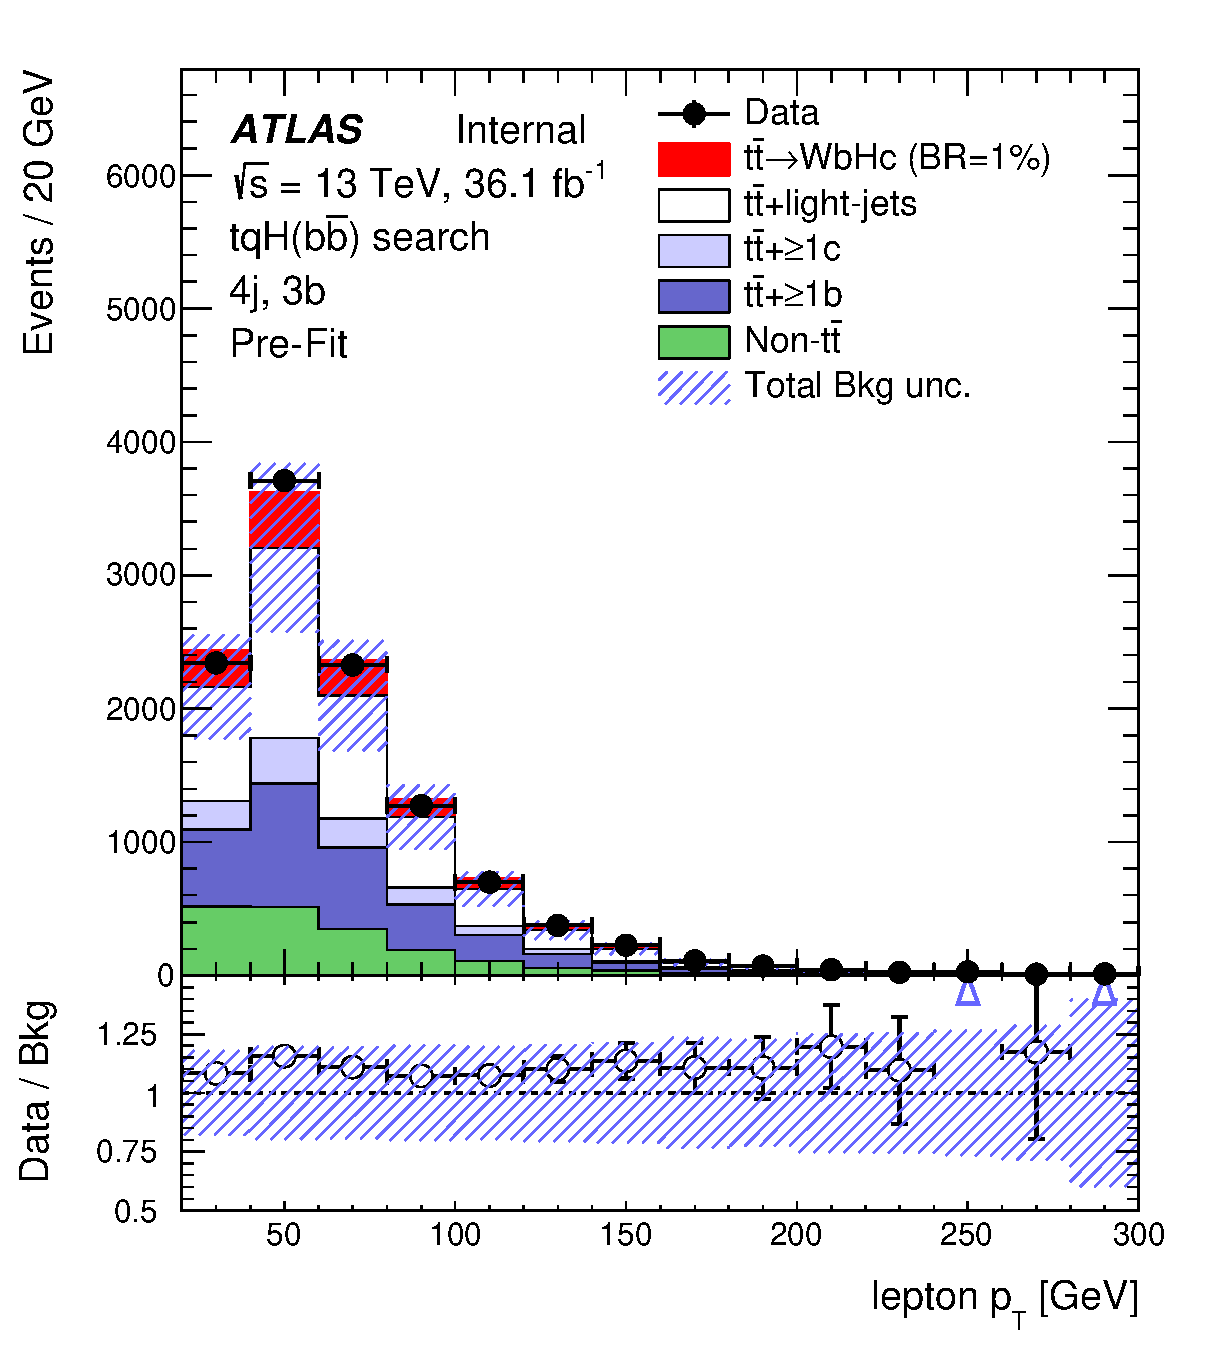
\includegraphics[width=0.40\textwidth]{figures/Hbb/other_variables/c1lep4jex3bex_lep0_pt.eps}}
\subfloat[]{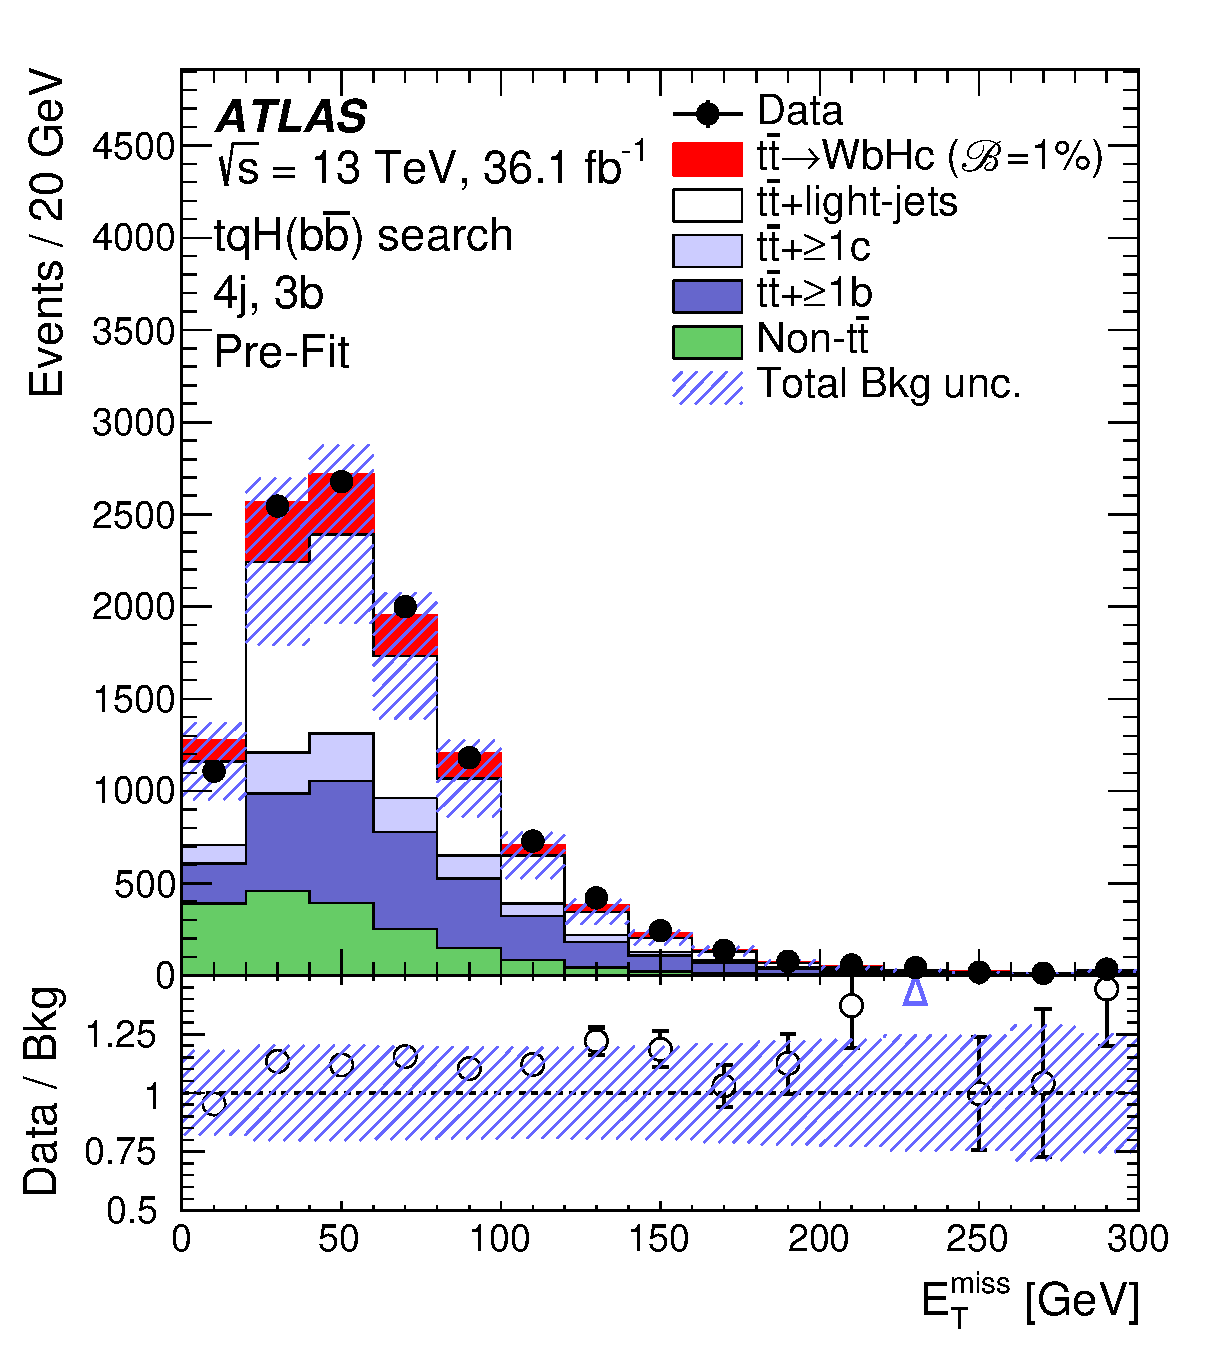
\includegraphics[width=0.40\textwidth]{figures/Hbb/other_variables/c1lep4jex3bex_met.eps}} \\
\subfloat[]{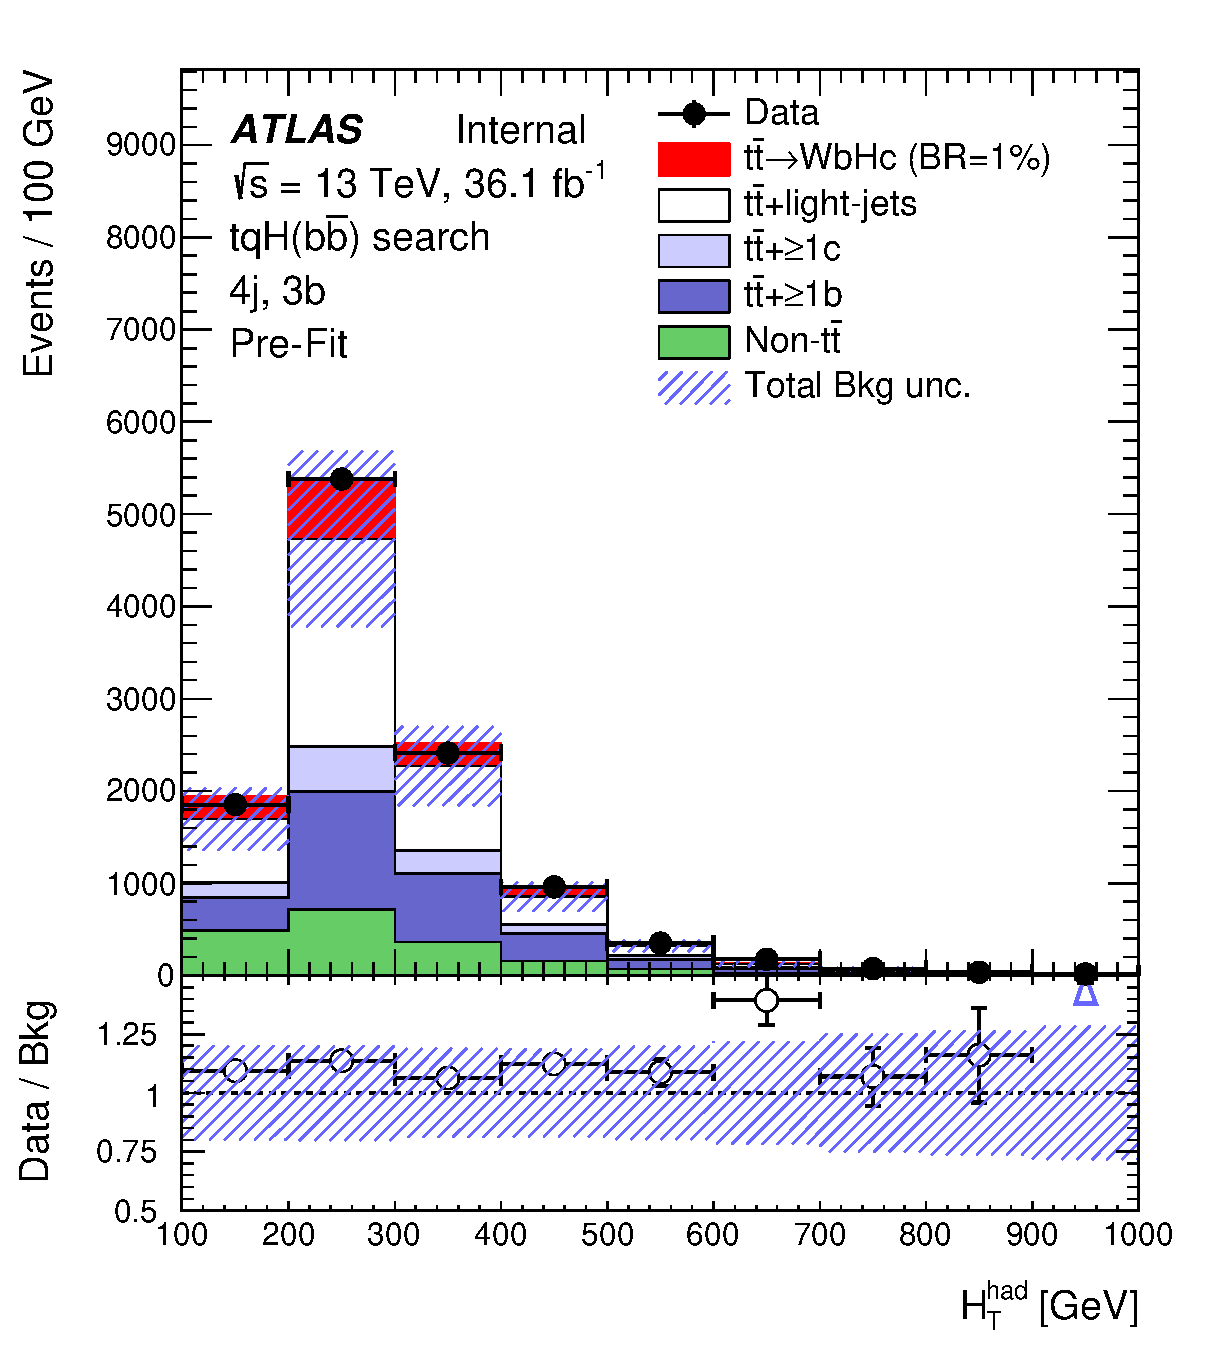
\includegraphics[width=0.40\textwidth]{figures/Hbb/other_variables/c1lep4jex3bex_hthad.eps}} 
\subfloat[]{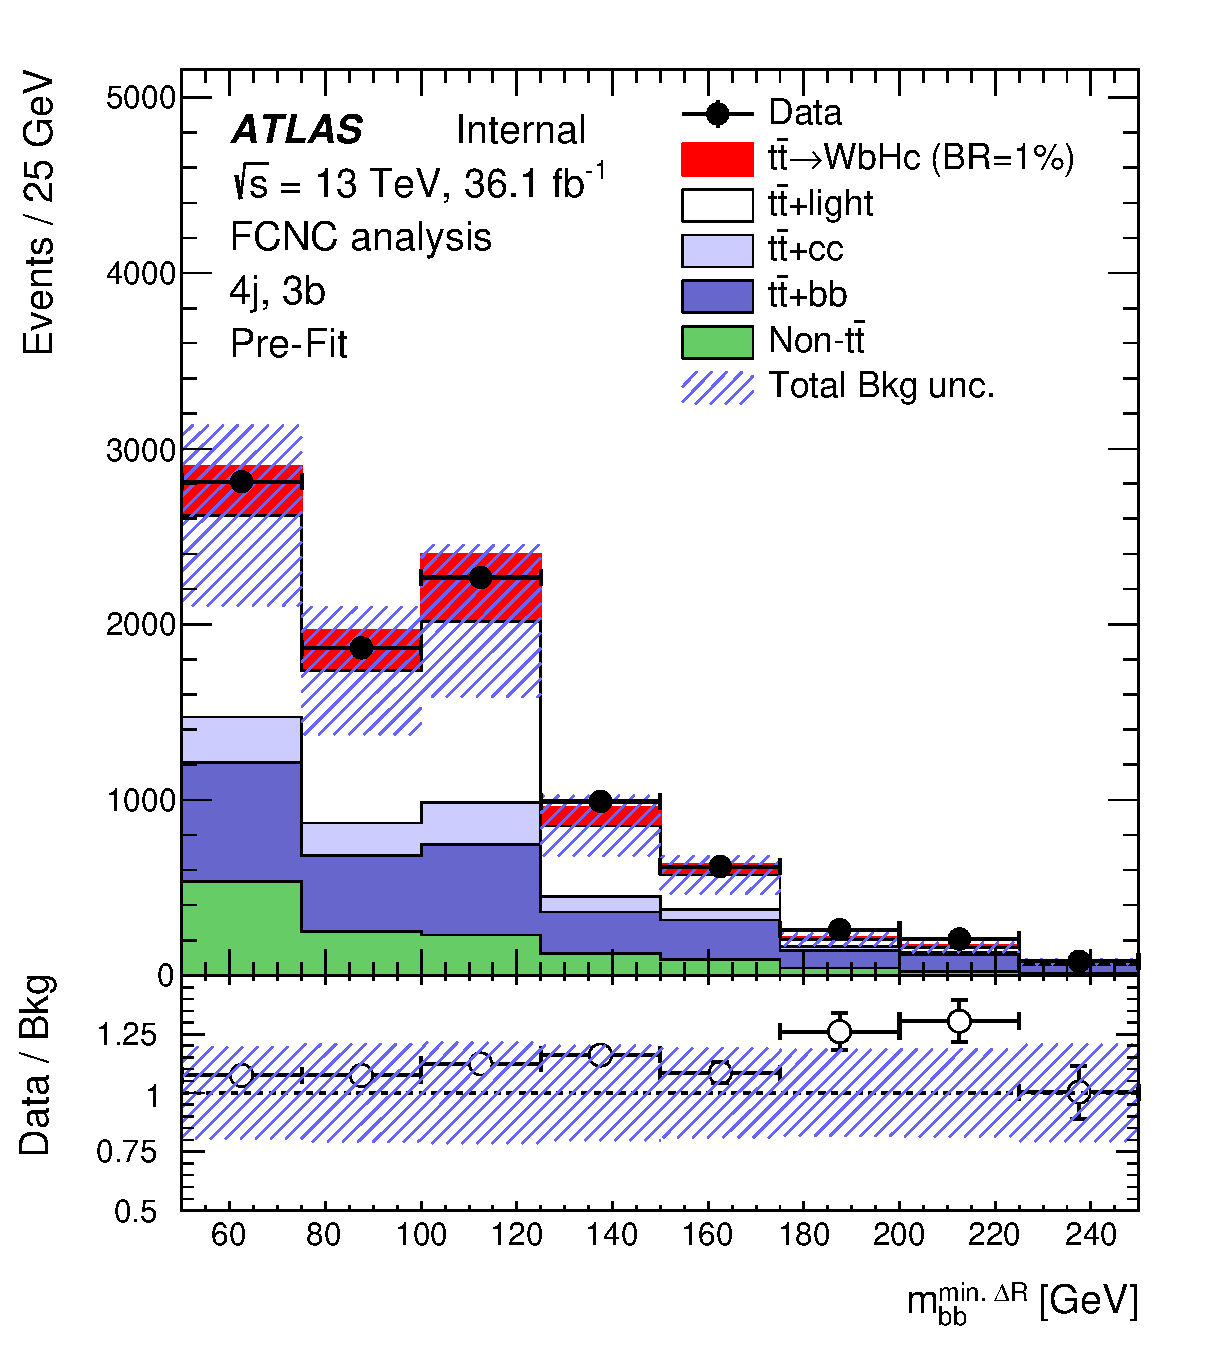
\includegraphics[width=0.40\textwidth]{figures/Hbb/other_variables/c1lep4jex3bex_mbb_mindR.eps}} \\ 
\caption{\small{$\Hbb$ search: Comparison between the data and background prediction for several kinematic 
distributions in the (4j, 3b) region before the fit to data (``Pre-Fit''). 
The distributions are shown for (a) lepton $\pt$, (b) $\met$, (c) scalar sum of the transverse momenta of 
the jets ($\hthad$), and (d) the invariant mass of the two $b$-tagged jets with lowest 
$\Delta R$ separation ($\mbb$).
The small contributions from $\ttbar V$, $\ttbar H$, single top, $W/Z$+jets, diboson, and multijet backgrounds are combined 
into a single background source referred to as ``Non-$\ttbar$''. 
The expected $\Hc$ signal (solid red) corresponding to $\BR(t\to Hc)=1\%$ is also shown,
added to the background prediction.
The last bin in all figures contains the overflow.
The bottom panel displays the ratio of data to the SM background (``Bkg'') prediction. 
The blue triangles indicate points that are outside the vertical range of the figure. 
The hashed area represents the total uncertainty of the background, excluding the normalisation uncertainty of the $\ttbin$ background, 
which is determined via a likelihood fit to data.}}
\label{fig:Hbb_extravars_4j3b}
\end{center}
\end{figure*}
%%%%%%%%%%%%%%%%%%%%%%%%%%%%%%%%%%%%%%%

%%%%%%%%%%%%%%%%%%%%%%%%%%%%%%%%%%%%%%%
\begin{figure*}[htbp]
\begin{center}
\subfloat[]{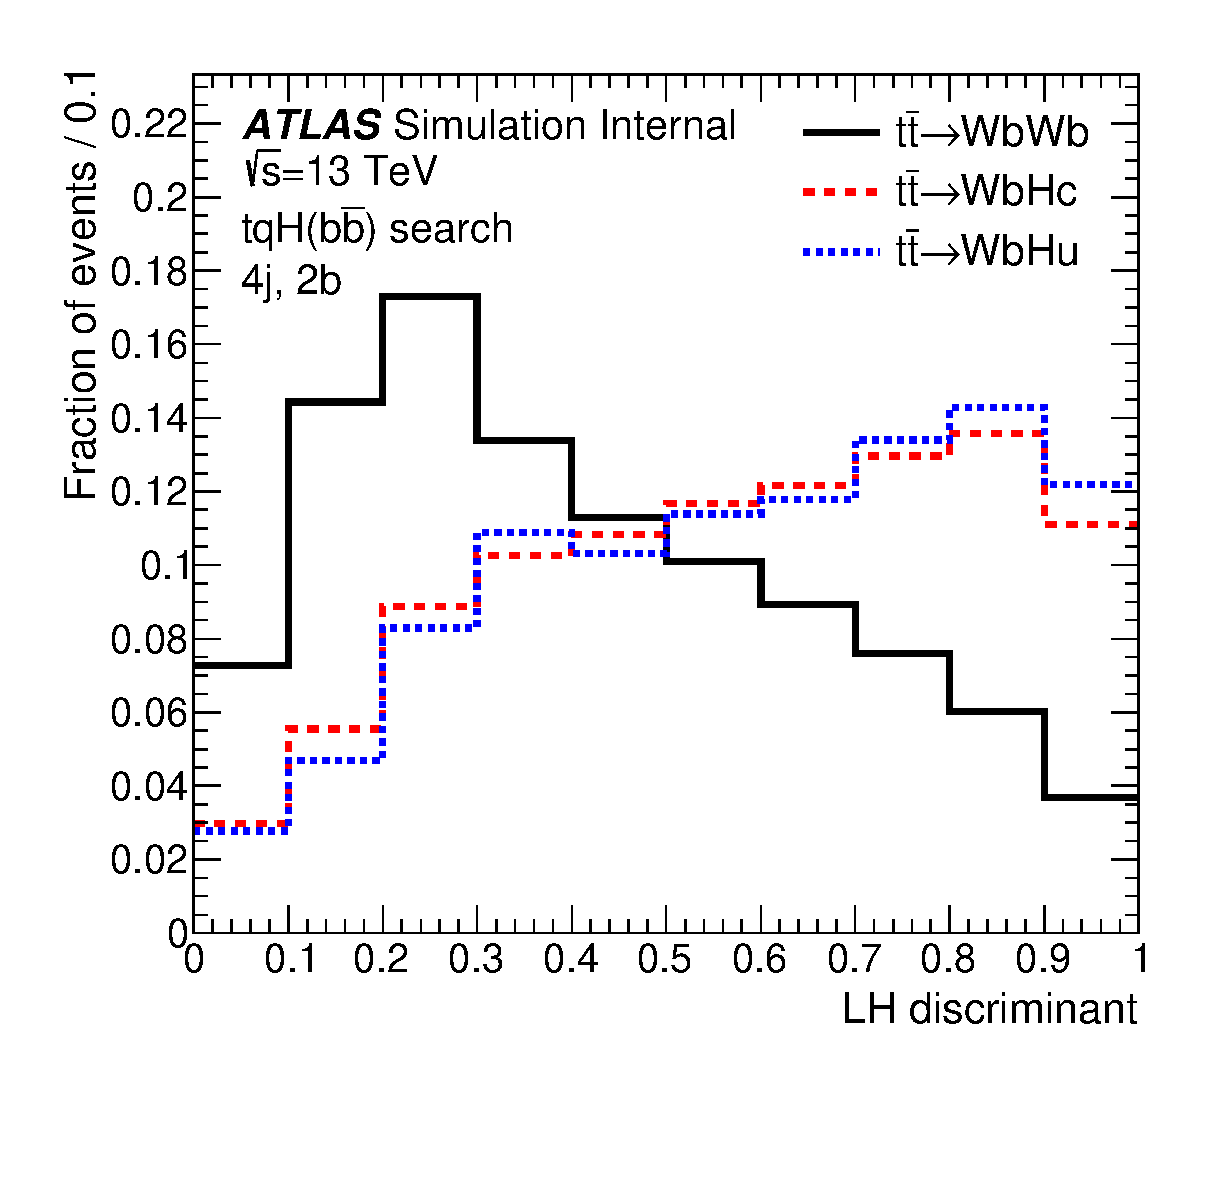
\includegraphics[width=0.33\textwidth]{figures/Hbb/discriminant_shape/canv_c1lep4jex2bex_FcncDiscriminant.eps}} 
\subfloat[]{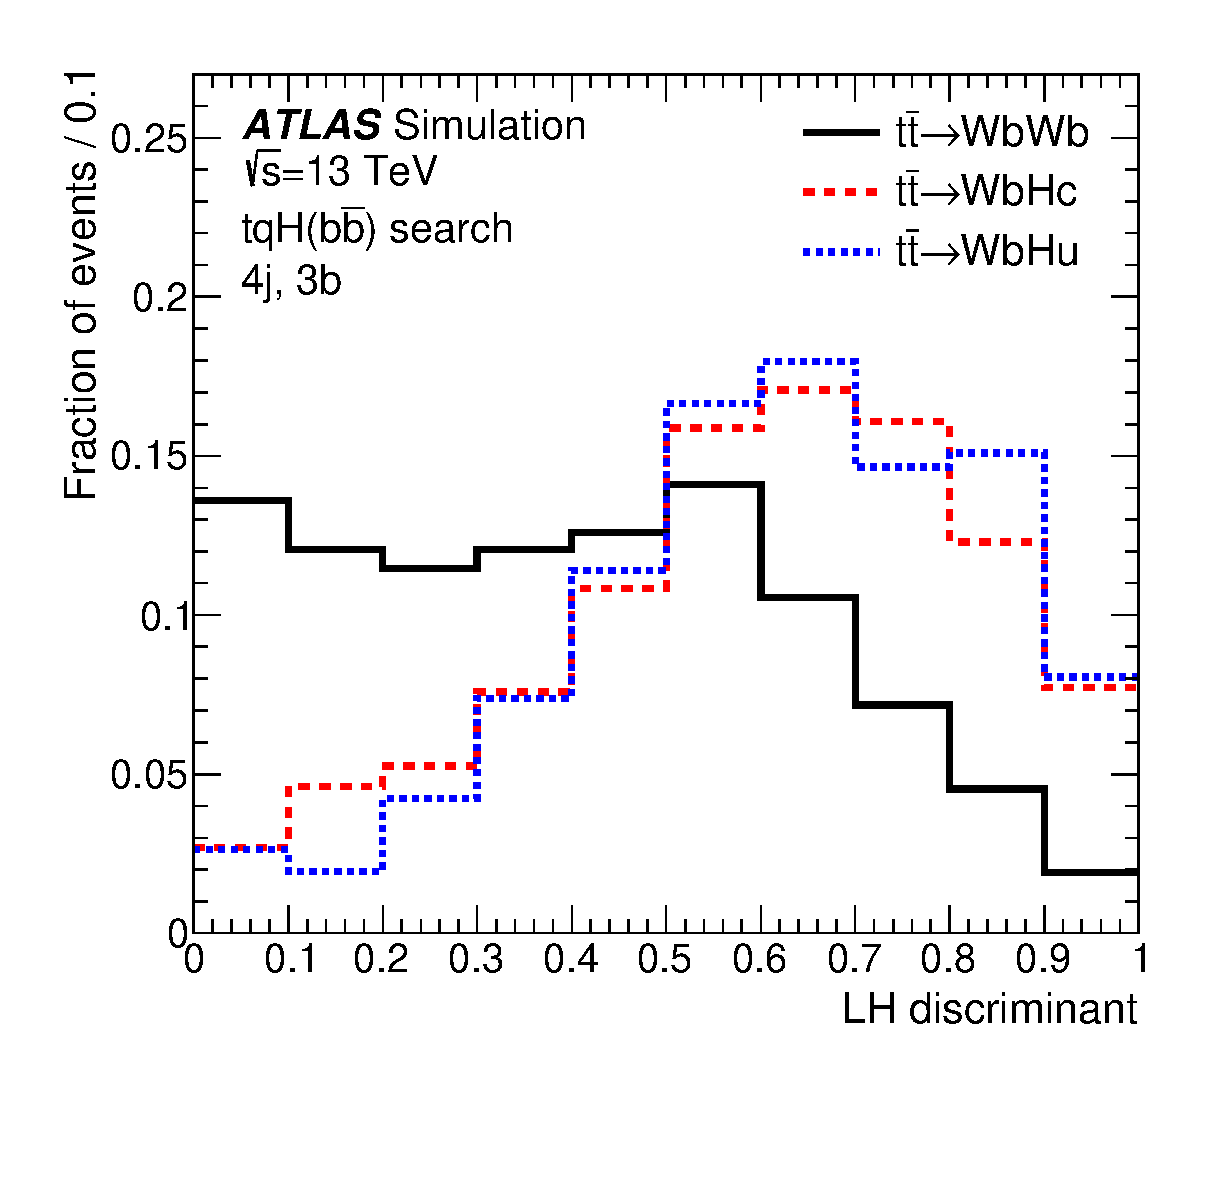
\includegraphics[width=0.33\textwidth]{figures/Hbb/discriminant_shape/canv_c1lep4jex3bex_FcncDiscriminant.eps}}
\subfloat[]{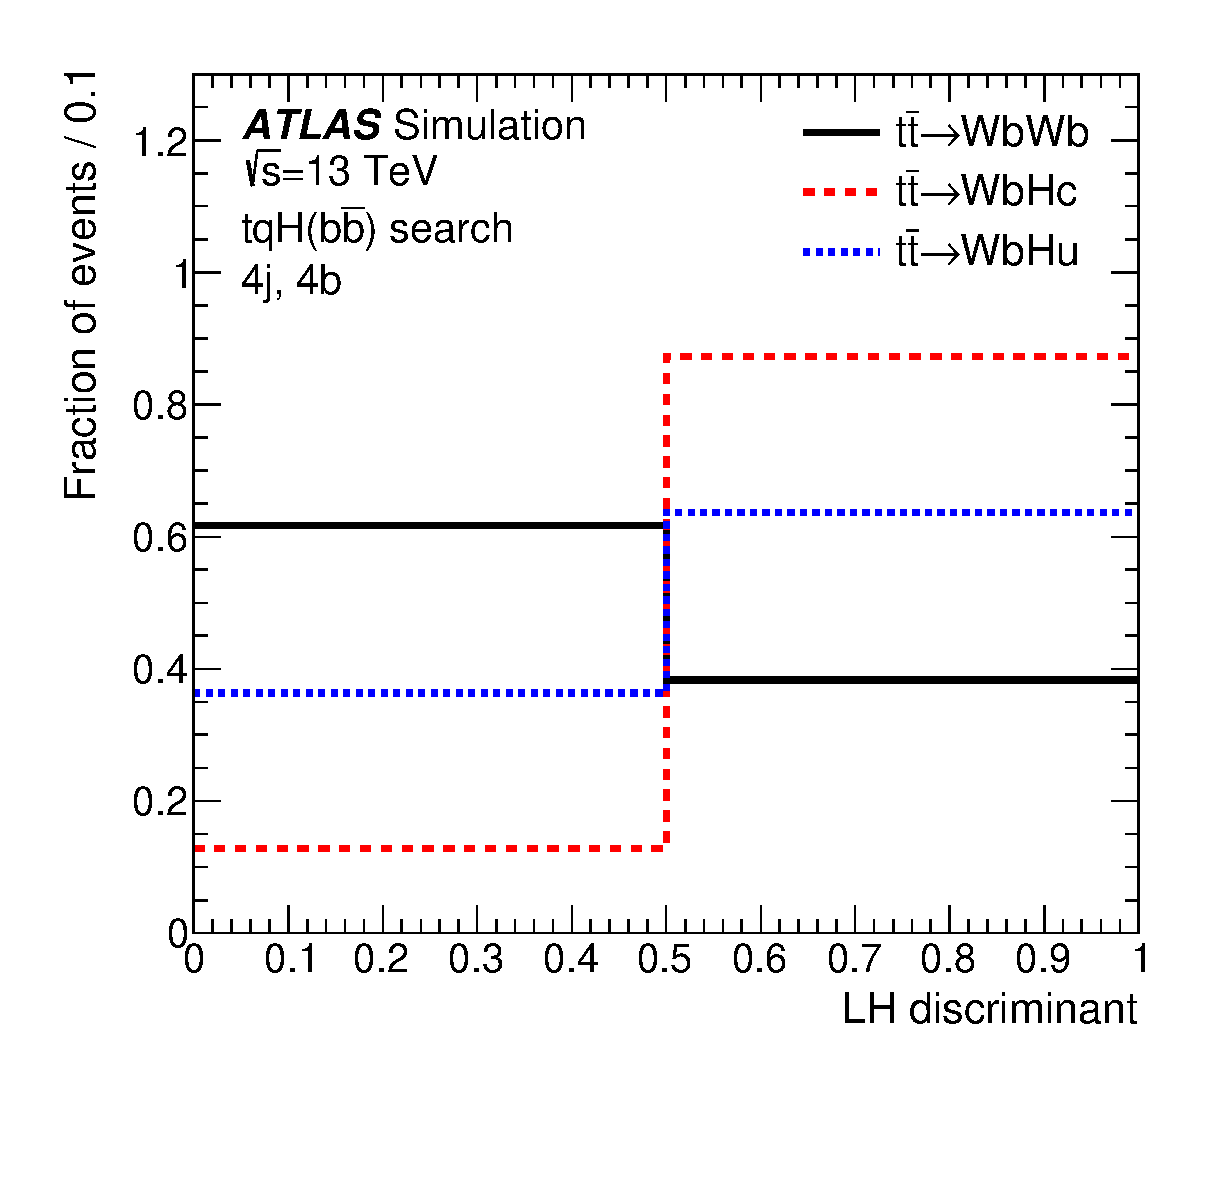
\includegraphics[width=0.33\textwidth]{figures/Hbb/discriminant_shape/canv_c1lep4jex4bin_FcncDiscriminant.eps}} \\
\subfloat[]{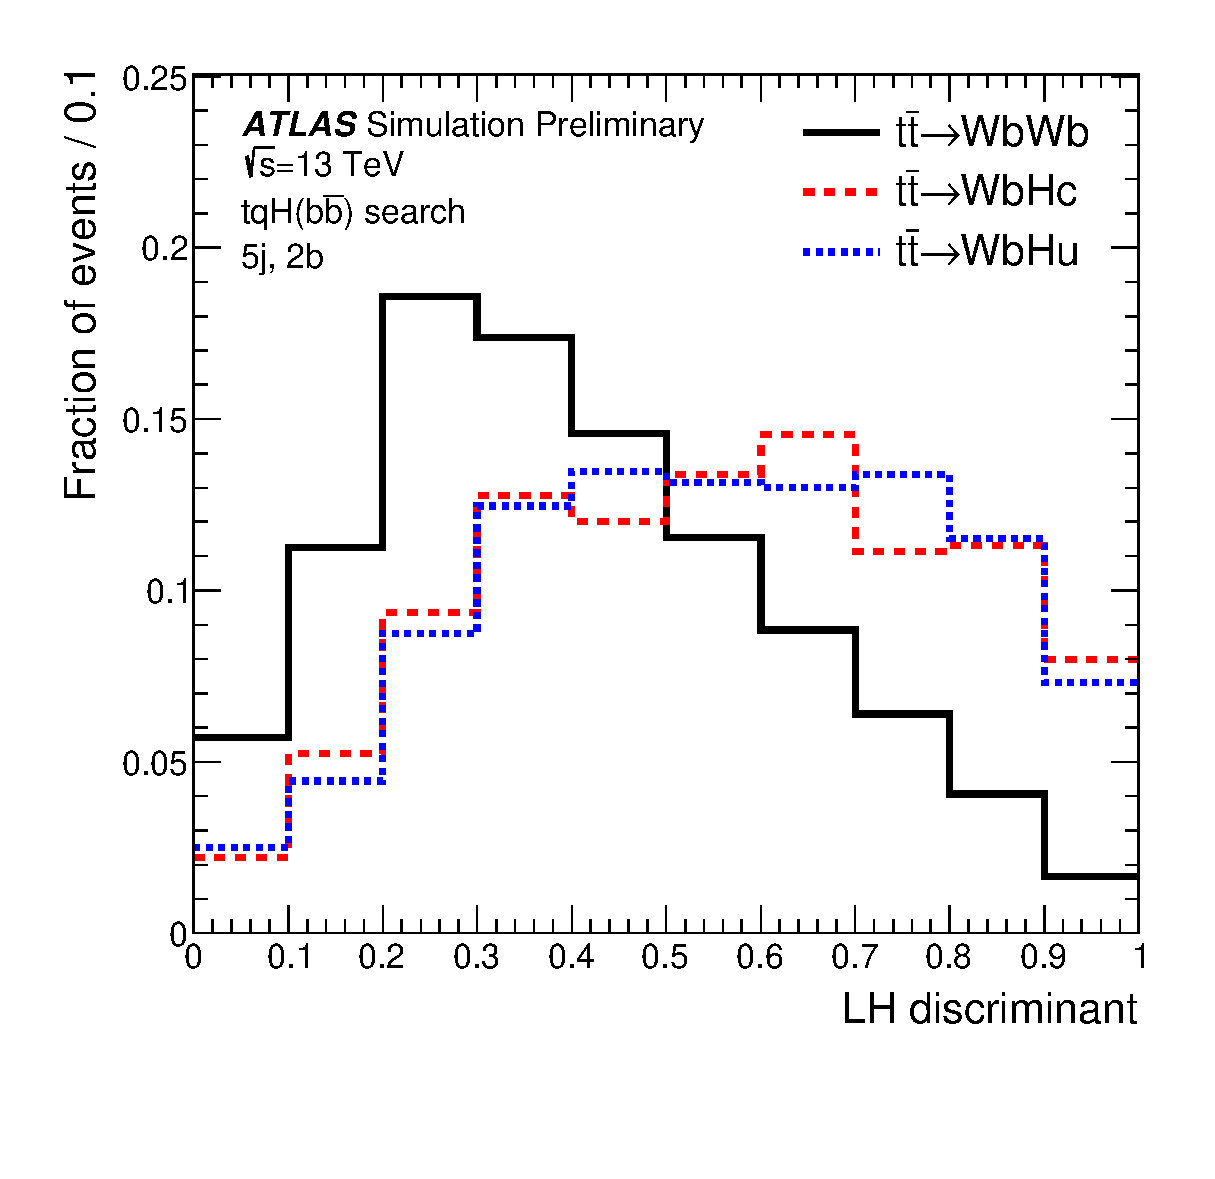
\includegraphics[width=0.33\textwidth]{figures/Hbb/discriminant_shape/canv_c1lep5jex2bex_FcncDiscriminant.eps}}
\subfloat[]{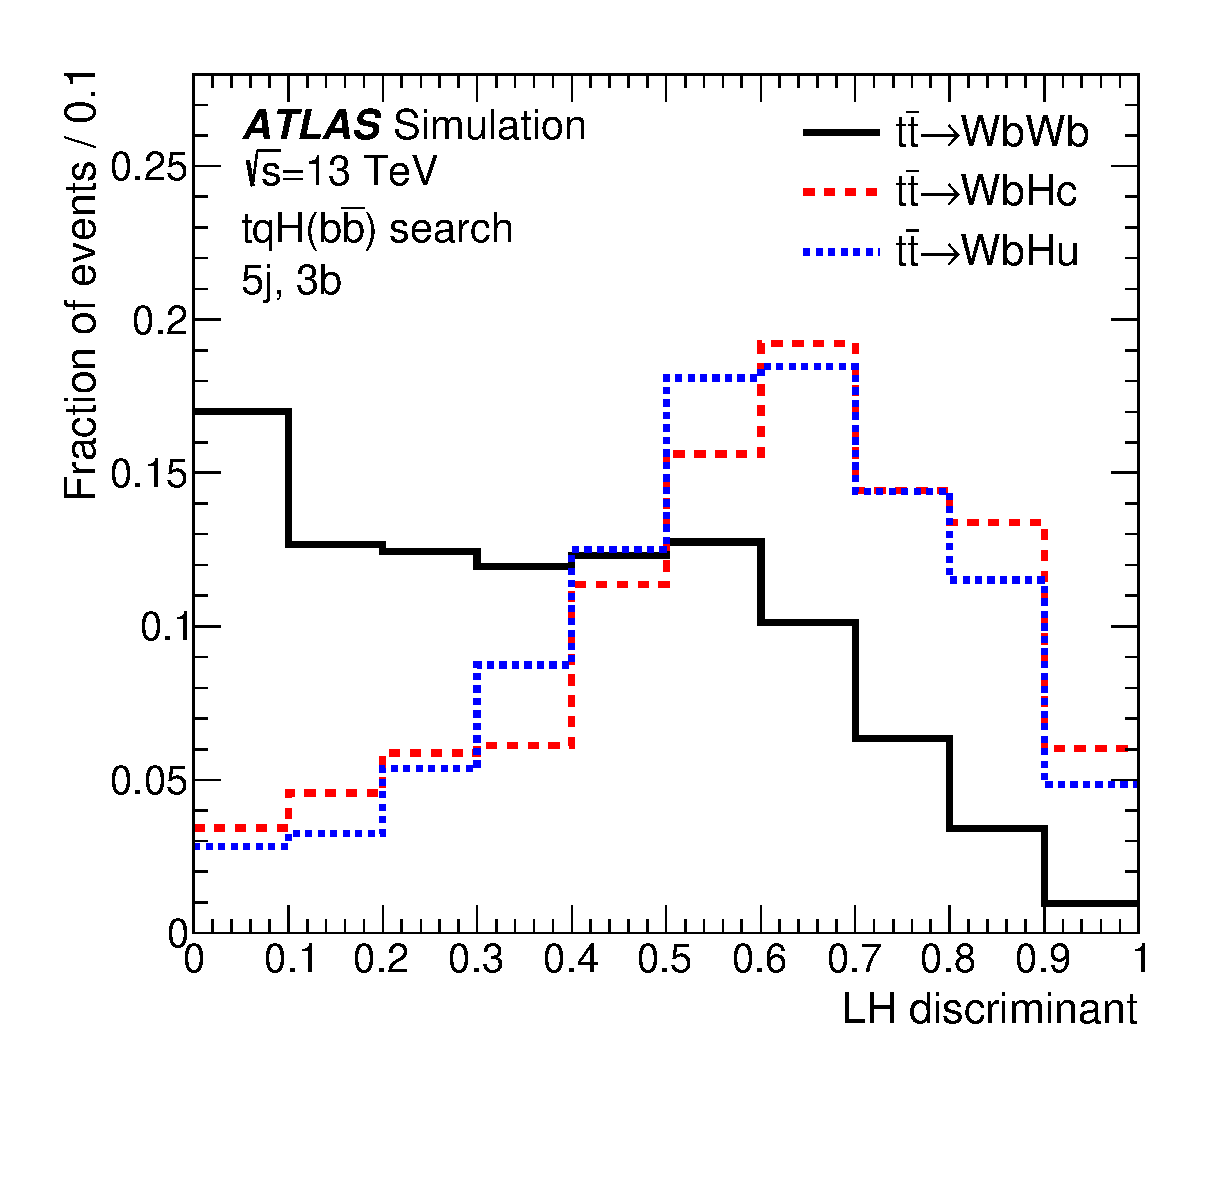
\includegraphics[width=0.33\textwidth]{figures/Hbb/discriminant_shape/canv_c1lep5jex3bex_FcncDiscriminant.eps}}
\subfloat[]{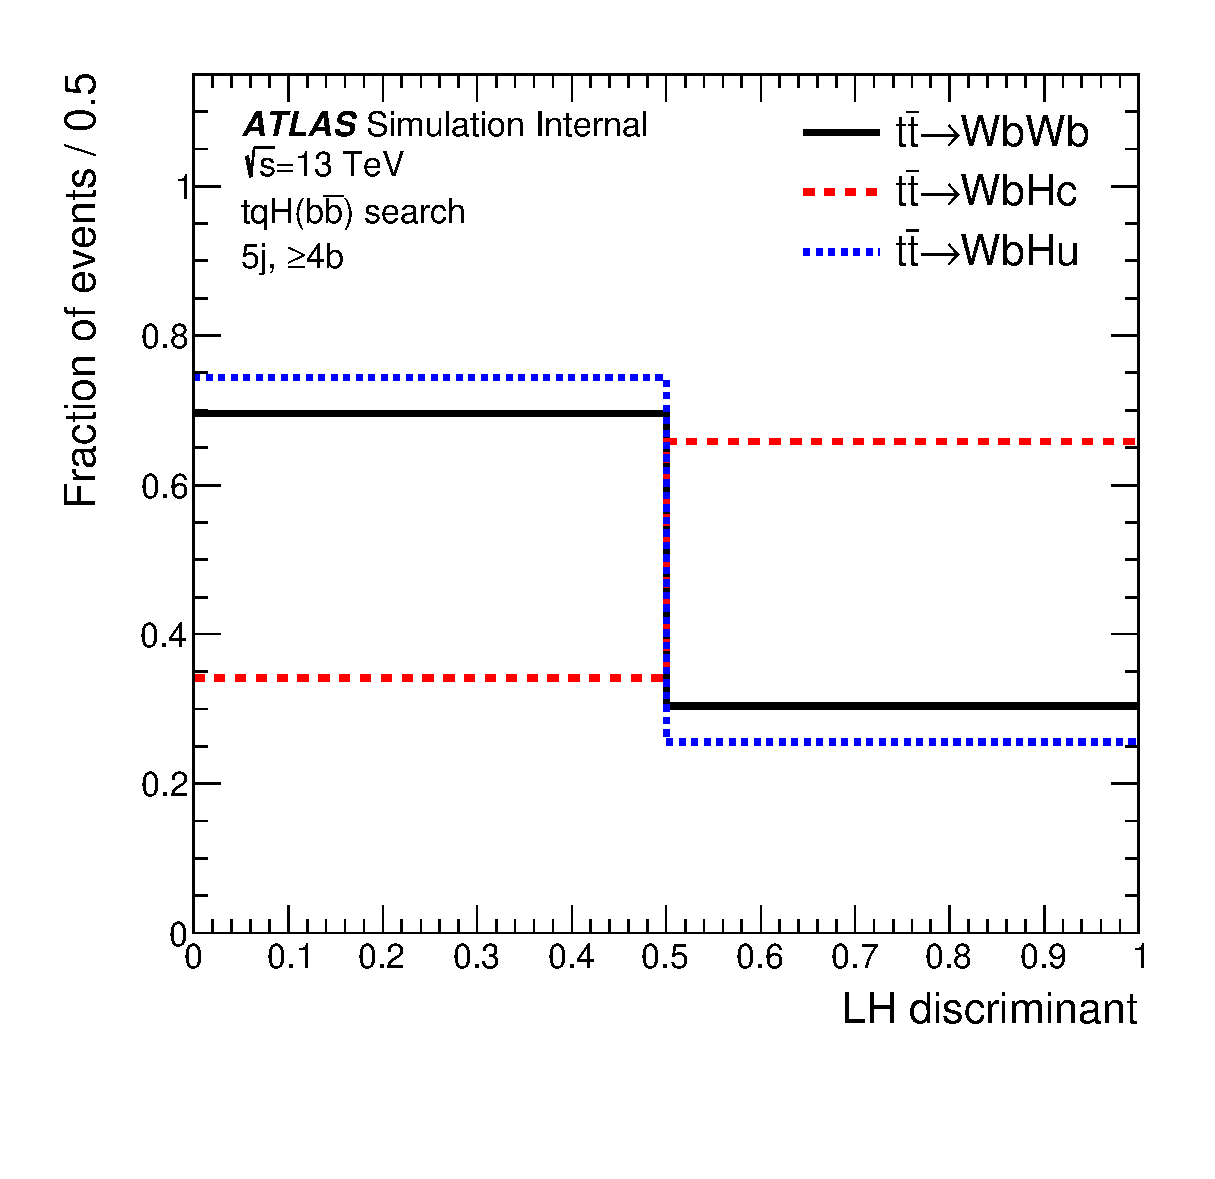
\includegraphics[width=0.33\textwidth]{figures/Hbb/discriminant_shape/canv_c1lep5jex4bin_FcncDiscriminant.eps}} \\
\subfloat[]{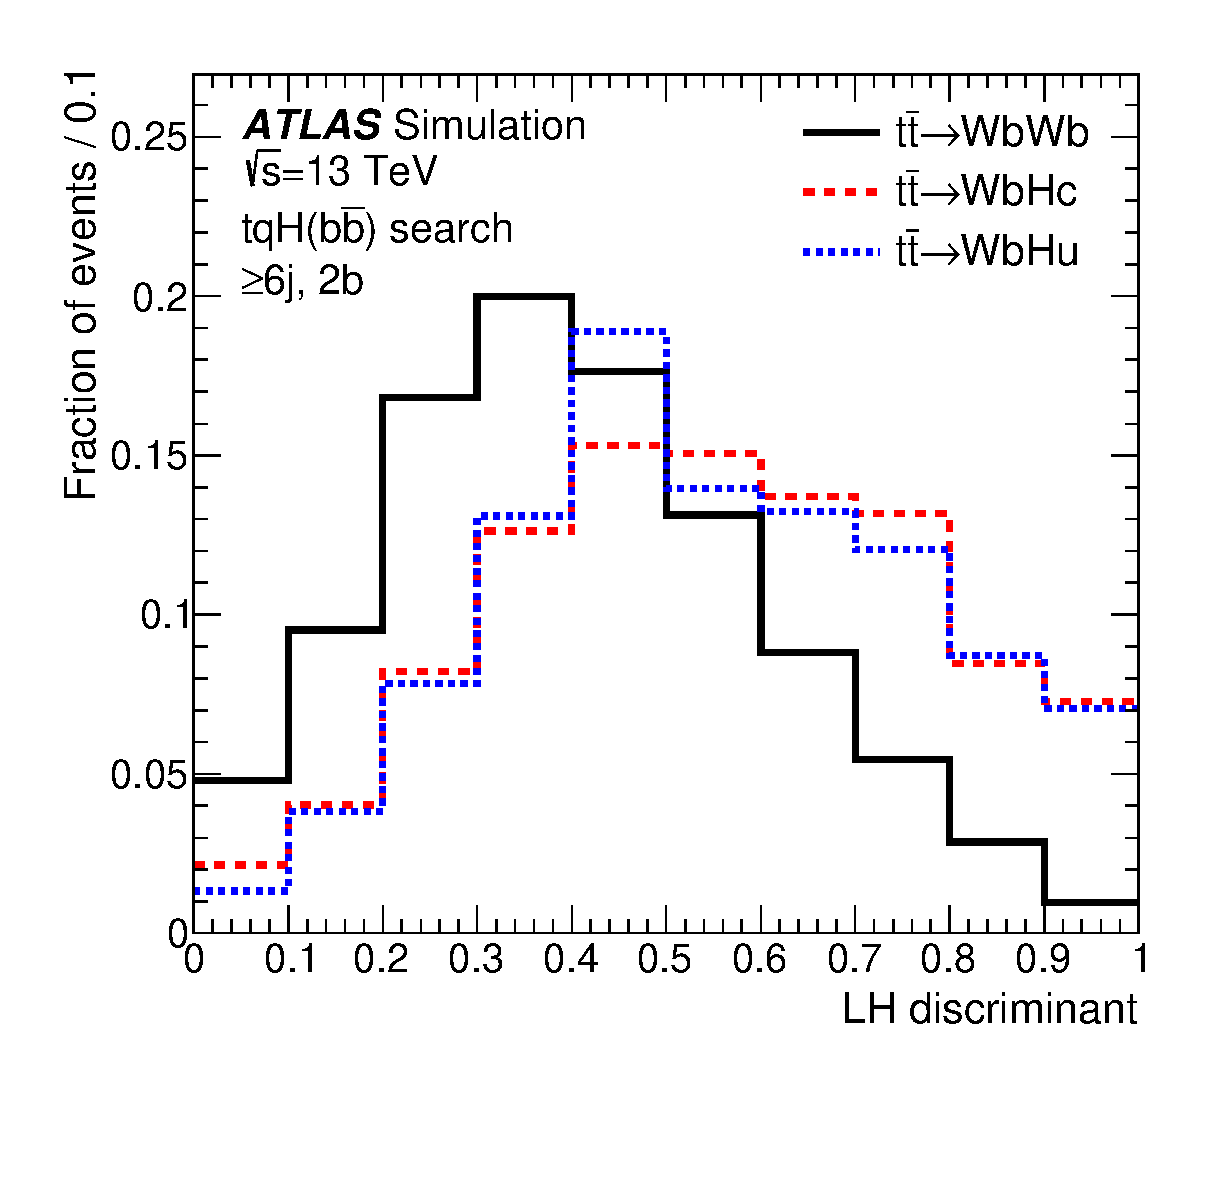
\includegraphics[width=0.33\textwidth]{figures/Hbb/discriminant_shape/canv_c1lep6jin2bex_FcncDiscriminant.eps}}
\subfloat[]{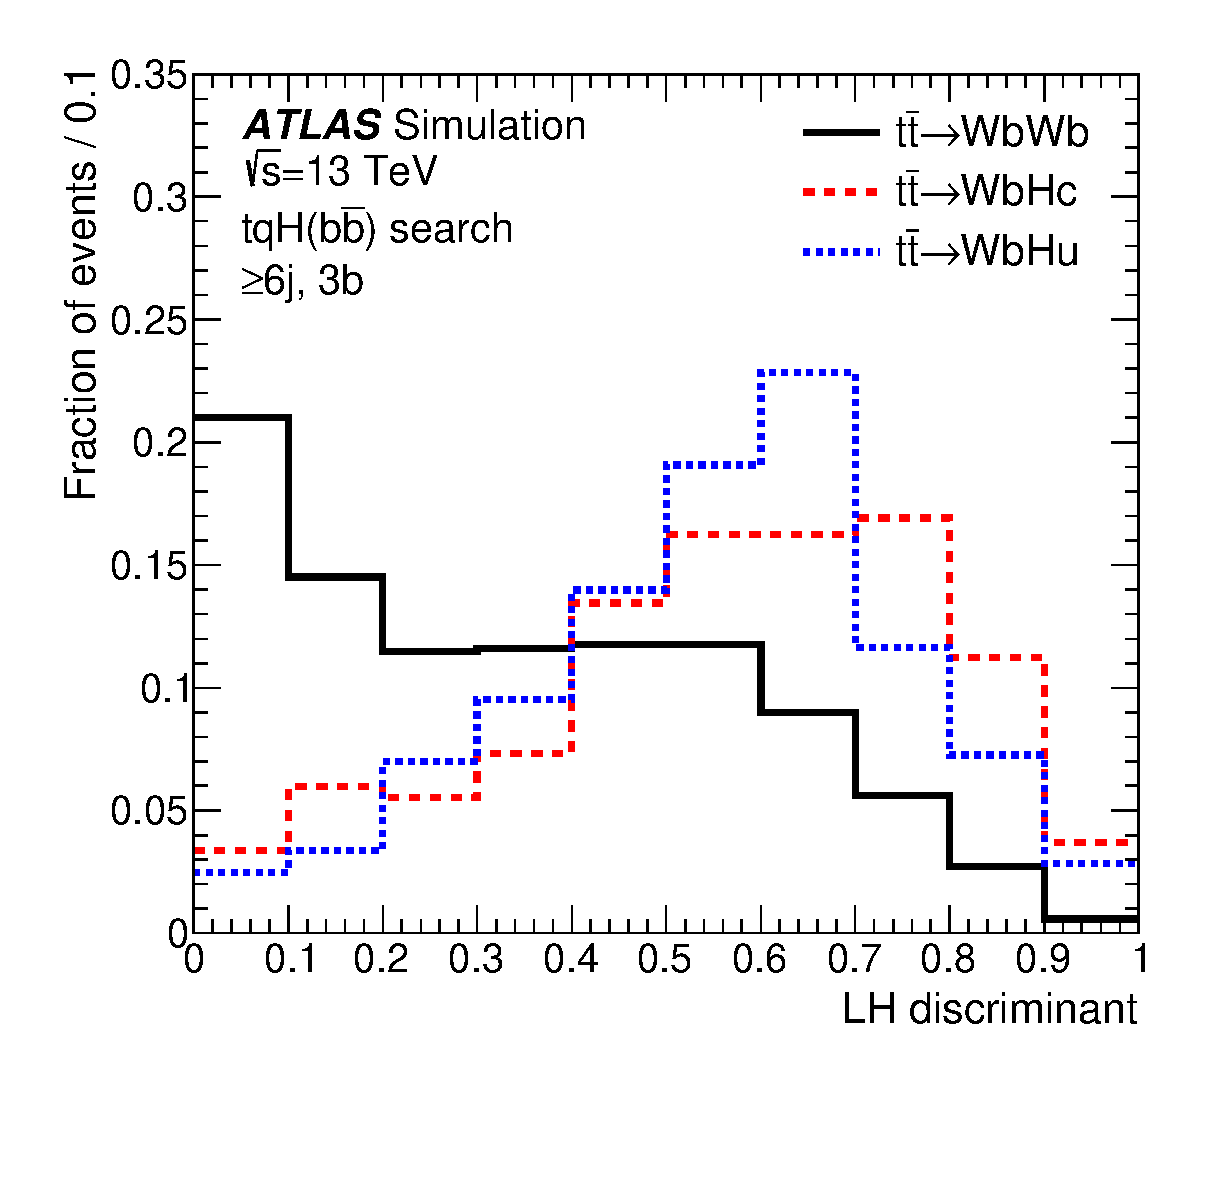
\includegraphics[width=0.33\textwidth]{figures/Hbb/discriminant_shape/canv_c1lep6jin3bex_FcncDiscriminant.eps}}
\subfloat[]{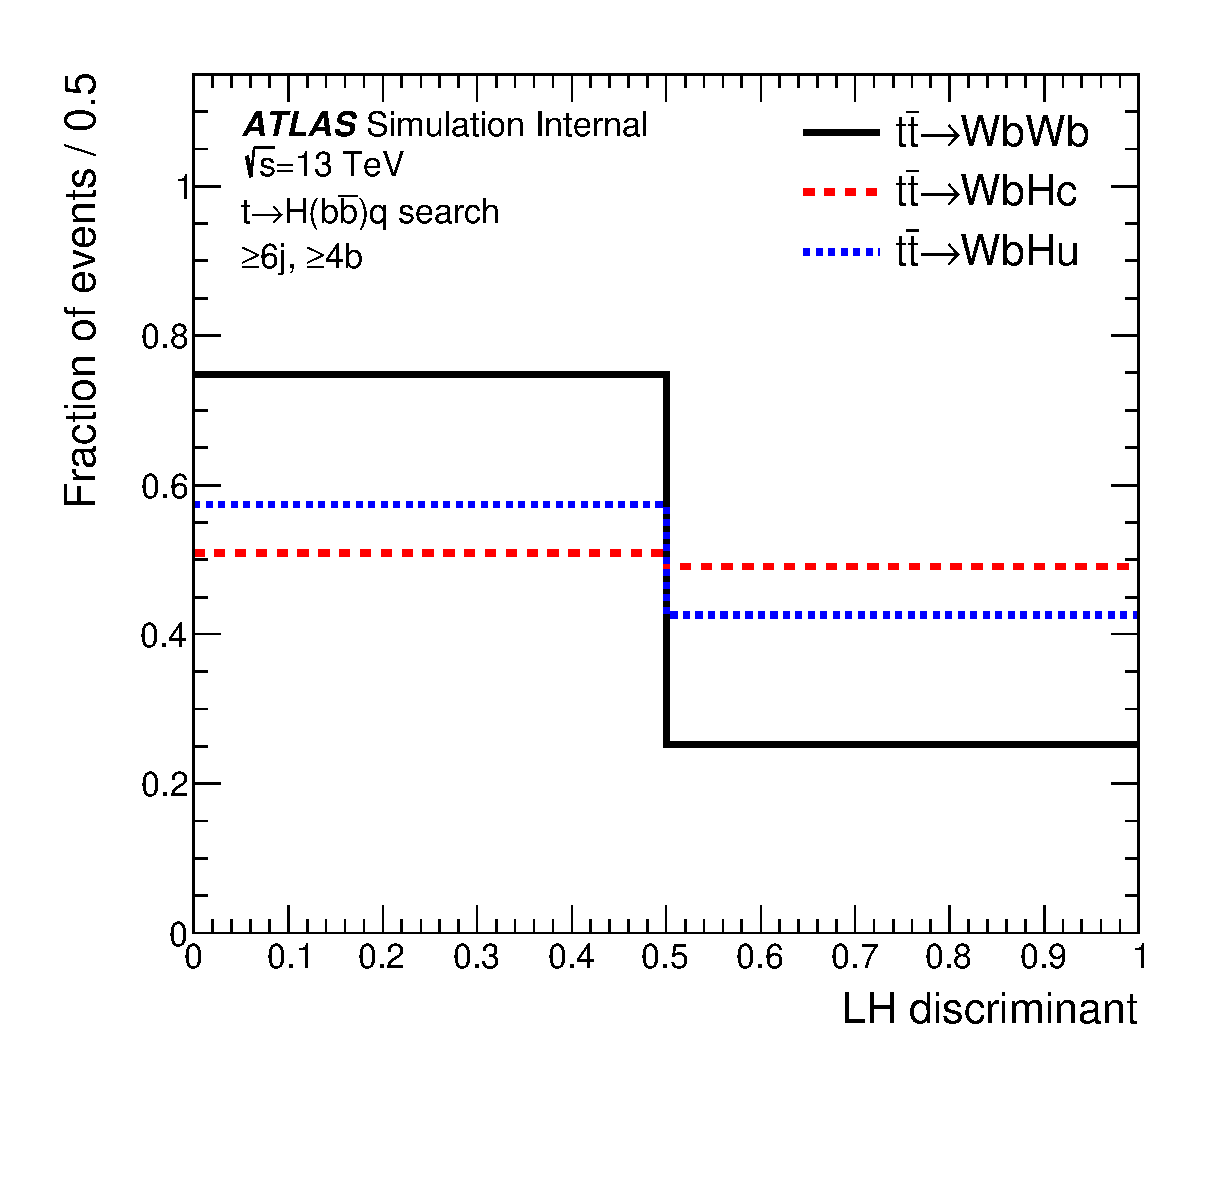
\includegraphics[width=0.33\textwidth]{figures/Hbb/discriminant_shape/canv_c1lep6jin4bin_FcncDiscriminant.eps}} \\
\caption{$\Hbb$ search: Comparison of the distributions of the LH discriminant after preselection 
between the $\Hc$ (red dashed) and $\Hu$ (blue dotted) signals, 
and the $t\bar{t}\to WbWb$ background (black solid) in different regions considered in the analysis:
(a) (4j, 2b), (b) (4j, 3b), (c) (4j, 4b), (d) (5j, 2b), (e) (5j, 3b), (f) (5j, $\geq$4b), (g) ($\geq$6j, 2b), 
(h) ($\geq$6j, 3b), and (i) ($\geq$6j, $\geq$4b). 
%Due to the small signal acceptance in 4b regions,
%which translates into low statistics for the simulated samples, only two bins are used for this distribution.
In the regions with $\geq$4 $b$-tagged jets, the signal acceptance is small, which translates
into low statistics for the simulated samples. Therefore, only two bins are used for these distributions.} 
\label{fig:LHD}
\end{center}
\end{figure*}
%%%%%%%%%%%%%%%%%%%%%%%%%%%%%%%%%%%%%%%%%%%%%%%%%% 



